\documentclass[tikz]{standalone}
\usetikzlibrary{positioning, arrows.meta}
\begin{document}
    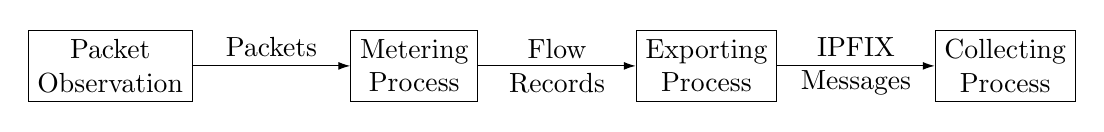
\begin{tikzpicture}[
        arrow/.style =  {-{Latex[length=1.5mm, width=1.0mm]},align=flush center}% 
    ]
        \node[draw, black, align=center] (capture) {Packet \\ Observation};
        \node[draw, black, right=2cm of capture, align=center] (metering) {Metering \\ Process};
        \node[draw, black, right=2cm of metering, align=center] (exporting) {Exporting \\ Process};
        \node[draw, black, right=2cm of exporting, align=center] (collecting) {Collecting \\ Process};

        \draw[arrow] (capture) -- (metering) node[midway,above] {Packets};
        \draw[arrow] (metering) -- (exporting) node[midway, align=center] {Flow \\ Records};
        \draw[arrow] (exporting) -- (collecting) node[midway, align=center] {IPFIX \\ Messages};
    \end{tikzpicture}
\end{document}